% Provenance (never printed): see sources/outline_sources.md (Year 3:
% Darcy's law; permeability; aquifer types; the groundwater-flow equation;
% pumping tests; solute transport, in principle).
% Brief: sources/book5/BRIEFS.md, ch. 23. Curves from figdata/bachelor-3/
% theis.py, flow_net.py and advection_dispersion.py; the site of Varden-3 from
% figdata/shared/region.py (read only). Exercise and problem values in the
% Book 5 scratch calculator calc/ch23.py. The wells, the dam, the tests and
% the solutes are invented.
\chapter{علم المياه الجوفية}\label{ch:b3:hydrogeology}

تضخّ بئرٌ جديدة \qty{2160}{m^3} من الماء يوميًا من الحجر الجيري الواقع على بُعد بضع
مئاتٍ من الأمتار تحت مزرعة. لا يطرأ شيء على بئر المزرعة نفسها
في البداية. وبعد شهر يقف ماؤها أدنى بنحو \qty{2}{m}، مع أنّها تبعد
كيلومترًا واحدًا، وأنّ محطة الضخّ لم تسحب منها قطرةً قطّ. منسوبُ
الماء حول البئر الجديدة لم ينخفض بانتظام، بل غاص في
مخروطٍ، وقد اتّسع المخروط بسرعة عبر صخرٍ يتحرّك فيه الماء
بنفسه بضعة سنتيمترات في اليوم. يبني هذا الفصل الفيزياء التي
تتنبأ بالرقمين معًا: الانتشار السريع للضغط والانتقال البطيء
للماء، انطلاقًا من قانون تجريبي واحد اكتُشف عام 1856.
% ledger: heath:darcy

\begin{recall}
المسامية، والنفاذية، ومنسوب المياه الجوفية، والمياه الجوفية، والخزانات الجوفية،
والينابيع والآبار واردة في كتب المدرسة، مع زمن مكوث الماء
والمياه الجوفية الأحفورية. وترد اللزوجة وقانون بوازوي لجريان السائل في أنبوب
ومعادلة الانتشار في كتب الفيزياء. أمّا دالة الخطأ
وحلول معادلة الانتشار التي تستعملها واردة في
الفصل~\ref{ch:b3:lithosphere-thermal-models}. تلال فاردن، المنطقة المختلقة
للسلسلة، بما فيها الحجر الرملي والحجر الجيري والطَّفل والطباشير، هي
منطقة التمارين منذ كتب المدرسة.
\end{recall}

\section{الحمل الهيدروليكي وقانون دارسي}\label{sec:b3:hydrogeology:darcy}

يتحرّك الماء الجوفي من حيث تكون طاقته الميكانيكية لكل وحدة وزن مرتفعة
إلى حيث تكون منخفضة. ولأنّه يتحرّك ببطء، فإنّ طاقته الحركية
مُهملة، وتتكوّن تلك الطاقة من جزأين: ارتفاع الماء
وضغطه.

\begin{definition}[الحمل الهيدروليكي؛ التدرّج الهيدروليكي]\label{def:b3:hydrogeology:head}
\emph{الحمل الهيدروليكي}\index{الحمل الهيدروليكي} عند نقطة من
الأرض المشبعة بالماء، ويُعطى بالعلاقة
\[
h = z + \frac{p}{\rho g} ,
\]
مجموع \emph{حمل الارتفاع} $z$ للنقطة فوق مستوى مرجعي
و\emph{حمل الضغط} $p/(\rho g)$، حيث $p$ ضغطُ الماء فوق
الضغط الجوي. وهو الارتفاع الذي يصعد إليه الماء في
أنبوب، أي مقياسٍ للضغط، مفتوحٍ عند تلك النقطة وحدها. و\emph{التدرّج
الهيدروليكي}\index{التدرّج الهيدروليكي} هو $\nabla h$؛ ومقداره بين نقطتين
تبعد إحداهما عن الأخرى مسافة $L$ على طول الانسياب، هو $\Delta h/L$.
\end{definition}

\begin{omfigure}
\centering
\begin{tikzpicture}[>=stealth, font=\small, x=1cm, y=1cm]
\fill[omLithAlluv!60] (0,-0.6) rectangle (7,3.2);
\fill[omSea!45] (0,-0.6) rectangle (7,1.9);
\draw[thick, brown!60!black] (0,3.2) -- (7,3.2);
\draw[omDef, dashed] (0,1.9) -- (7,1.9);
\node[omDef, font=\scriptsize, anchor=south east] at (6.9,1.92) {منسوب المياه الجوفية};
% piezometer
\fill[white] (3.3,0.4) rectangle (3.7,4.0);
\draw[thick] (3.3,0.7) -- (3.3,4.0); \draw[thick] (3.7,0.7) -- (3.7,4.0);
\draw[thick, densely dotted] (3.3,0.4) -- (3.3,0.7); \draw[thick, densely dotted] (3.7,0.4) -- (3.7,0.7);
\fill[omSea!70] (3.32,0.4) rectangle (3.68,2.6);
\draw[omDef, thick] (3.3,2.6) -- (3.7,2.6);
\fill (3.5,0.55) circle (0.06);
\node[font=\scriptsize, anchor=west] at (3.75,0.55) {\foreignlanguage{arabic}{المصفاة، عند النقطة $P$}};
% datum
\draw[black!60] (0,-0.6) -- (7,-0.6);
\node[font=\scriptsize, anchor=north west] at (0,-0.62) {\foreignlanguage{arabic}{المستوى المرجعي، $z = 0$}};
% heads, on the left of the tube
\draw[<->] (2.5,-0.6) -- node[left, font=\scriptsize] {$z$} (2.5,0.55);
\draw[<->] (2.5,0.55) -- node[left, font=\scriptsize] {$p/\rho g$} (2.5,2.6);
\draw[black!40, densely dashed] (2.4,0.55) -- (3.3,0.55);
\draw[black!40, densely dashed] (1.0,2.6) -- (3.3,2.6);
\draw[<->, thick, omThm] (1.1,-0.6) -- node[left, font=\scriptsize] {$h$} (1.1,2.6);
\node[font=\scriptsize, anchor=south] at (3.5,4.0) {مقياس الضغط};
\end{tikzpicture}

\par\smallskip{\small مقياس الضغط، وهو أنبوب مفتوح عند مصفاته فقط. يقف
الماء فيه عند \omterm{def:b3:hydrogeology:head}{الحمل الهيدروليكي} للنقطة $P$، أي ارتفاع
$z$ مضافًا إليه حمل الضغط. وهنا يكون المستوى في الأنبوب أعلى من
منسوب المياه الجوفية، كما هو الحال حيث يصعد الماء نحو الينبوع أو
نهرٍ.}\label{fig:b3:hydrogeology:head}
\end{omfigure}

في عام 1856 قاس هنري دارسي، المهندس الفرنسي، تدفّق الماء عبر
أعمدةٍ من الرمل، ووجده متناسبًا مع فقد الحمل لكل
وحدة طول. والجريان صفائحيّ: يتبع الماء خطوط انسياب منفصلة.
% ledger: heath:darcy

\begin{theorem}[قانون دارسي]\label{thm:b3:hydrogeology:darcy}
في وسط مسامي مشبع، يكون حجم الماء العابر وحدة المساحة في
وحدة الزمن هو
\[
\vec q = -K\,\nabla h ,
\]
حيث $K$ يعتمد على الوسط وعلى المائع. وفي وسطٍ تكون مساماته
أنابيبَ مستقيمةً متوازيةً نصف قطرها $a$ تشغل كسرًا $n$ من
الحجم، يعطي قانون بوازوي هذا القانون مع
\[
K = \frac{k\rho g}{\mu}, \qquad k = \frac{na^2}{8} ,
\]
حيث $\mu$ لزوجةُ الماء.
\end{theorem}
\index{قانون دارسي}

\begin{proof}
العبارة الأولى هي \omterm{thm:b3:hydrogeology:darcy}{قانون دارسي} التجريبي. في أنبوبٍ نصف قطره $a$
على طول الانسياب، يعطي قانون بوازوي متوسط السرعة $\bar u =
-(a^2/8\mu)\,\mathrm d(p + \rho gz)/\mathrm dl = -(a^2\rho g/8\mu)\,\mathrm
dh/\mathrm dl$، لأنّ $p + \rho gz = \rho g h$. وتشغل الأنابيب
الكسر $n$ من أيّ مقطع عرضي، إذن حجم الماء لكل وحدة مساحة كلية هو
$q = n\bar u = -(na^2/8)(\rho g/\mu)\,\mathrm dh/\mathrm dl$.
\end{proof}

ليست المسامُ الحقيقية أنابيبَ مستقيمةً؛ فالمبرهنة تبيّن صورة القانون
وكيفية تغيّره مع الأبعاد. ويتناسب الانسياب طرديًّا مع التدرّج ومع مربّع حجم
المسام، ويتناسب عكسيًّا مع اللزوجة: فالرمل نفسه يسمح للماء بالمرور أسرع
عندما يكون دافئًا.

\begin{definition}[التصريف النوعي؛ الموصلية الهيدروليكية؛ النفاذية الذاتية]\label{def:b3:hydrogeology:darcy}
\emph{التصريف النوعي}\index{التصريف النوعي} $\vec q$ هو
حجم الماء الذي يعبر وحدة المساحة من الوسط، الحبيبات والمسام
معًا، في وحدة الزمن. \emph{الموصلية
الهيدروليكية}\index{الموصلية الهيدروليكية} $K$ هو معامل
\omterm{thm:b3:hydrogeology:darcy}{قانون دارسي}، بوحدة \unit{m/s} أو \unit{m/d}. \emph{النفاذية
الذاتية}\index{النفاذية الذاتية} للوسط هي $k =
K\mu/(\rho g)$، بوحدة \unit{m^2}: وهي تعتمد على الوسط وحده.
\end{definition}

تمتدّ \omterm{def:b3:hydrogeology:darcy}{الموصلية الهيدروليكية} للصخور عبر اثنتي عشرة رتبةً من
المقدار، كما تفعل قلّةٌ من الكميات الفيزيائية. ويُقرأ من مخطّط مسحٍ كلاسيكي
للموضوع، ويكون المدى النموذجي بالأمتار في اليوم كالتالي: الطين
\num{e-7} إلى \num{e-4}؛ الغرين والليس \num{e-3} إلى 2؛ الرمل الغريني 0.04 إلى
10؛ الرمل النظيف 0.3 إلى 150؛ الحصى 100 إلى 4000؛ الطَّفل \num{e-8} إلى
\num{e-4}؛ الحجر الرملي \num{e-5} إلى 0.4؛ الصخور الكربوناتية \num{e-4} إذا كانت
متشقّقة فقط، وتبلغ عدّة آلاف إذا كانت مغارية؛ والصخور النارية
والمتحوّلة تقلّ عن \num{e-8} إذا كانت غير متشقّقة، وتصل إلى بضعة
متشقّقة. كما تنقل معظم الصخور الماء على طول طبقاتها أفضل مما
تنقله عبرها.
% ledger: heath:darcy, heath:k-chart

\omterm{def:b3:hydrogeology:darcy}{التصريف النوعي} هو دفقٌ عبر المساحة كلّها؛ فالماء يجري
عبر المسام فقط، وبسرعة أكبر.

\begin{definition}[سرعة التسرّب]\label{def:b3:hydrogeology:seepage}
\emph{سرعة التسرّب}\index{سرعة التسرّب} هي $\vec v = \vec
q/n_e$، متوسط سرعة الماء في المسام، حيث $n_e$ هي
المسامية الفعّالة، وهي مسامية المسام المتّصلة التي يجري فيها
الماء.
\end{definition}

رملٌ خشنٌ ذو $K = \qty{60}{m/d}$ وتدرّجٌ قدره 1 في 1000،
ومسامية قدرها 0.20 يتحرّك ماؤه بسرعة \qty{0.3}{m/d}؛ وفي طينٍ ذي $K =
\qty{e-4}{m/d}$، وتدرّج قدره 1 في 10 ومسامية قدرها 0.50، بسرعة
\qty{2e-5}{m/d}، أي أقل من سنتيمتر في السنة. لا تجري المياه الجوفية
في أنهارٍ جوفيةٍ، إلّا في كهوف الحجر الجيري وأنابيب
الحمم. وهذه متوسطات: فحيثما ينتقل ملوّث، قد يسير جزؤه الأسرع
أسرع بعدّة مرّات.
% ledger: heath:velocity

\section{الخزانات الجوفية}\label{sec:b3:hydrogeology:aquifers}

\begin{definition}[الخزانات الجوفية المحصورة وغير المحصورة؛ الطبقة شبه الكتيمة]\label{def:b3:hydrogeology:aquifer-types}
\emph{الخزان الجوفي غير المحصور}\index{الخزان الجوفي غير المحصور} هو خزانٌ جوفيّ
سطحُه العلويّ هو منسوب المياه الجوفية. أمّا \emph{الخزان الجوفي
المحصور}\index{الخزان الجوفي المحصور} هو خزانٌ تعلوه طبقةٌ ذات
موصليةٍ أقلّ بكثير، بحيث يكون الماء فيه تحت ضغط: ففي بئرٍ
يصل إليه، يرتفع الماء فوق قمّة الخزان، إلى
سطحه البيزومتري. والطبقة ذات الموصلية المنخفضة التي تُبطئ مرور الماء دون أن
توقفه بين الخزانات الجوفية هي
\emph{الطبقة شبه الكتيمة}\index{الطبقة شبه الكتيمة}.
\end{definition}

\begin{definition}[الناقلية؛ معامل التخزين؛ الإنتاجية النوعية]\label{def:b3:hydrogeology:storage}
\emph{الناقلية}\index{الناقلية} للخزان الجوفي ذي السُّمك
$b$ هي $T = Kb$، أي التدفّق لكل وحدة عرض تحت تدرّج الوحدة، بوحدة
\unit{m^2/d}. أمّا \emph{معامل التخزين}\index{معامل التخزين}
(أو معامل التخزين) $S$ فهو حجم الماء المنطلق لكل وحدة مساحة من
الخزان عندما ينخفض الحمل بوحدة واحدة؛ وهو عديم البعد.
و\emph{الإنتاجية النوعية}\index{الإنتاجية النوعية} $S_y$ للصخر فهو حجم
الماء الذي يتصرّف منه بفعل الجاذبية لكل وحدة حجم عندما ينخفض
منسوب المياه الجوفية خلاله.
\end{definition}

يُطلق نوعا الخزانات الجوفية الماء بطريقتين مختلفتين. ففي \omterm{def:b3:hydrogeology:aquifer-types}{الخزان الجوفي
المحصور} ينخفض الحمل لكن المسام تبقى ممتلئة: يتمدّد الماء قليلًا،
والخزان، إذ يحمل جزءًا أكبر من وزن الصخور فوقه،
يُضغط قليلًا. ويُطلق تمدّد الماء وحده نحو
\num{9e-7} متر مكعب لكل متر مكعب من الخزان ولكل متر من الحمل؛
ومع الانضغاط، يكون \omterm{def:b3:hydrogeology:storage}{معامل التخزين} لمعظم الخزانات المحصورة
\num{e-5} إلى \num{e-3}. أمّا في الخزان غير المحصور فينخفض منسوب المياه الجوفية
وتُفرَّغ المسام الواقعة فوقه: \omterm{def:b3:hydrogeology:storage}{فمعامل التخزين} هو \omterm{def:b3:hydrogeology:storage}{الإنتاجية النوعية}، نحو 0.1
إلى 0.3، أي أكبر منه بمائة إلى عشرة آلاف مرّة. وتتراوح ناقلية الخزانات
المستعملة من أقلّ من \qty{1}{m^2/d} في الصخور المتشقّقة
إلى \qty{100000}{m^2/d} في الحجر الجيري المغاري وتدفّقات الحمم. وحيثما
يُسحب حمل الخزان المحصور لزمنٍ طويل، فيُفرَّغ الطين الموجود فيه وحوله من الماء
ويتراصّ، فتهبط الأرض فوقه.
% ledger: heath:storage, heath:transmissivity

\begin{omfigure}
\centering
\begin{tikzpicture}[>=stealth, font=\small, x=1cm, y=1.1cm]
\begin{scope}
\clip (0,-1.3) -- (0,2.0) -- (3.5,2.9) -- (5,3.5) -- (7.5,4.2) -- (11,3.8) -- (11,-1.3) -- cycle;
\fill[lith sandstone] (0,-1.3) rectangle (11,4.5);
\fill[lith limestone] (0,1.8) -- (11,-0.95) -- (11,0.05) -- (0,2.8) -- cycle;
\fill[lith shale] (0,2.8) -- (11,0.05) -- (11,1.25) -- (0,4.0) -- cycle;
\fill[omLithLime!25] (0,4.0) -- (11,1.25) -- (11,4.5) -- (0,4.5) -- cycle;
\end{scope}
\draw[thick, brown!60!black] (0,2.0) -- (3.5,2.9) -- (5,3.5) -- (7.5,4.2) -- (11,3.8);
% water table in the chalk
\draw[omDef, dashed, thick] (4.5,3.0) .. controls (6,3.35) and (8.5,3.35) .. (11,2.8);
\node[omDef, font=\scriptsize, anchor=south] at (6.6,3.32) {منسوب المياه الجوفية};
% potentiometric surface of the limestone
\draw[omThm, densely dashdotted, thick] (1.4,2.36) -- (11,2.2);
\node[omThm, font=\scriptsize, anchor=south east, fill=white, inner sep=1pt] at (10.9,2.25) {السطح البيزومتري للحجر الجيري};
% well Varden-3
\draw[thick] (2.9,2.74) -- (2.9,1.05); \draw[thick] (3.1,2.8) -- (3.1,1.05);
\fill[omDef!35] (2.92,1.05) rectangle (3.08,2.33);
\draw[omThm, thick] (2.85,2.33) -- (3.15,2.33);
\node[font=\scriptsize, anchor=south] at (3.0,2.95) {\foreignlanguage{arabic}{فاردن-3}};
% labels
\node[font=\scriptsize, fill=white, inner sep=1pt] at (7.5,0.45) {الحجر الجيري: الخزان الجوفي المحصور};
\node[font=\scriptsize, fill=white, inner sep=1pt] at (7.5,1.5) {الطَّفل: الطبقة الحاصرة};
\node[font=\scriptsize, fill=white, inner sep=1pt] at (8.4,2.8) {الطباشير: الخزان الجوفي غير المحصور};
\node[font=\scriptsize, fill=white, inner sep=1pt] at (7.5,-0.8) {الحجر الرملي};
\node[font=\scriptsize, fill=white, inner sep=1pt, align=center] at (0.8,1.75) {الحجر الجيري\\الانكشاف};
\draw[->, omDef, thick] (0.8,3.0) -- (0.8,2.3);
\node[omDef, font=\scriptsize, anchor=south] at (0.8,3.0) {التغذية};
\end{tikzpicture}

\par\smallskip{\small مقطع تخطيطي لغطاء تلال فاردن
من الغرب إلى الشرق، غير مرسوم بمقياس. يحتوي الطباشير على خزان جوفي غير محصور
تحت منسوب المياه الجوفية فيه. يُغذّى الحجر الجيري الجوراسي حيث
ينكشف، ويكون محصورًا تحت الطَّفل: في البئر فاردن-3 من
المسألة، المحفورة عبر الطَّفل والمفتوحة على الحجر الجيري وحده، فإنّ
الماء يرتفع إلى السطح الكموني، أعلى بكثير من قمة
الخزان الجوفي لكنه أدنى من سطح الأرض.}\label{fig:b3:hydrogeology:aquifers}
\end{omfigure}
% ledger: region:name

\section{معادلة انسياب المياه الجوفية}\label{sec:b3:hydrogeology:flow-equation}

\begin{theorem}[معادلة انسياب المياه الجوفية]\label{thm:b3:hydrogeology:flow-equation}
في خزان جوفي محصور ذي ناقلية ثابتة $T$ ومعامل تخزين $S$،
بانسياب أفقي، يحقّق الحمل $h(x, y, t)$
\[
S\,\frac{\partial h}{\partial t} = T\nabla^2h + W ,
\]
$W$ حجم الماء المضاف إلى وحدة المساحة في وحدة الزمن بالتغذية أو
المسحوب بالضخّ (سالب). وفي الانسياب المستقرّ بلا منابع، $\nabla^2h =
0$.
\end{theorem}
\index{معادلة انسياب المياه الجوفية}

\begin{proof}
خُذ عمودًا من الخزان الجوفي مساحته $\mathrm dx\,\mathrm dy$. ويُحسب الانسياب لكلّ
وحدة عرض عبر سمكه الكامل $-T\nabla h$، \omterm{thm:b3:hydrogeology:darcy}{بقانون دارسي}
مضروبًا في $b$. صافي التدفّق الداخل هو $-\nabla\cdot(-T\nabla h)\,\mathrm dx\,\mathrm
dy = T\nabla^2h\,\mathrm dx\,\mathrm dy$. ويتغيّر الماء المخزّن في العمود
بمعدّل $S\,(\partial h/\partial t)\,\mathrm dx\,\mathrm dy$،
بحسب تعريف $S$. وبانحفاظ الكتلة، مع اعتبار كثافة الماء ثابتة في الموازنة،
يُساوي التخزين التدفّق الداخل زائدًا المنابع.
\end{proof}

هي معادلة الانتشار الواردة في كتب الفيزياء، مع الانتشارية الهيدروليكية
$T/S$ بدلًا من الانتشارية الحرارية. ففي حجر جيري محصور ذي
$T = \qty{450}{m^2/d}$ و$S = \num{2e-4}$ تبلغ الانتشارية
\qty{2.25e6}{m^2/d}: ينتشر تغيّر الحمل عبر \qty{1}{km} خلال
زمنًا نحو $L^2S/T$، أي نصف يوم. والحجر الجيري نفسه غير المحصور، ذو $S =
0.2$، يستغرق زمنًا أطول بألف مرة. ينتشر الضغط بسرعة، أمّا
الماء فيتحرّك ببطء: الرقمان الواردان في المقدّمة.

\begin{proposition}[انسياب شعاعي مستقرّ نحو بئر]\label{prop:b3:hydrogeology:thiem}
تضخّ بئرٌ $Q$ من خزان جوفي محصور ذي ناقلية $T$، ويكون الانسياب
مستقرًّا وشعاعيًّا. بين مسافتين $r_1 < r_2$ عن البئر،
تختلف قيمتا الانخفاض بمقدار
\[
s_1 - s_2 = \frac{Q}{2\pi T}\ln\frac{r_2}{r_1} .
\]
\end{proposition}

\begin{proof}
عبر كلّ دائرة نصف قطرها $r$ حول البئر يكون التدفّق الداخل $Q = 2\pi r
T\,\mathrm dh/\mathrm dr$. بالتكامل $\mathrm dh = (Q/2\pi T)\,\mathrm
dr/r$ من $r_1$ إلى $r_2$، وبكتابة $s = h_0 - h$، نحصل على النتيجة.
\end{proof}

في بعدين، يُرسم الانسياب المستقرّ \omterm{def:b3:hydrogeology:flow-net}{بشبكة الانسياب}.

\begin{definition}[شبكة الانسياب]\label{def:b3:hydrogeology:flow-net}
\emph{شبكة الانسياب}\index{شبكة الانسياب} هي رسم لانسياب المياه الجوفية المستقرّ في
مقطعٍ متجانسٍ متساوي الخواص بعائلتين من المنحنيات: خطوط تساوي الكمون،
أي خطوط الحمل المتساوي، وخطوط الانسياب التي يتّبعها الماء. 
تتقاطع خطوط الانسياب مع خطوط تساوي الكمون بزوايا قائمة، وفي شبكة الانسياب
تتباعد بحيث تكون الخلايا مربّعات منحنية الأضلاع.
\end{definition}

\begin{method}[التسرّب من شبكة الانسياب]\label{met:b3:hydrogeology:flow-net}
\leavevmode
\begin{enumerate}
\item ارسم الحدود: الحدّ غير النافذ هو خطّ انسياب، وقاع جسم
  مائي، حيث يكون الحمل ثابتًا، هو خطّ تساوي كمون.
\item ارسم $N_d$ من فروق الحمل بين أعلى حمل وأدنى حمل، $\Delta h
  = H/N_d$، وخطوط الانسياب التي تُشكّل $N_f$ قناة انسياب، بالتجربة،
  حتى تصبح كلّ خلية مربّعًا منحني الأضلاع.
\item تحمل كلّ قناة $K\Delta h$ لكلّ وحدة طول عمودية على
  المقطع، فيُحذف طول المربّع وعرضه، ويكون المجموع $q =
  KHN_f/N_d$.
\end{enumerate}
\end{method}

\begin{omfigure}
\centering
\begin{tikzpicture}
\begin{axis}[width=0.95\linewidth, height=0.36\linewidth, axis equal image,
  xmin=-60, xmax=60, ymin=-20, ymax=13, xlabel={\mbox{\textdir TLT $x$ (\unit{m})}}, ylabel={\mbox{\textdir TLT $z$ (\unit{m})}},
  tick label style={font=\scriptsize}, label style={font=\small}, clip=false]
% computed in figdata/bachelor-3/flow_net.py
\fill[omLithAlluv!35] (axis cs:-60,-20) rectangle (axis cs:60,0);
\fill[omSea!40] (axis cs:-60,0) rectangle (axis cs:-10,11.2);
\fill[omSea!40] (axis cs:10,0) rectangle (axis cs:60,1.2);
\fill[black!35] (axis cs:-10,0) -- (axis cs:-10,12.5) -- (axis cs:-5,12.5) -- (axis cs:10,0) -- cycle;
\pgfplotsinvokeforeach{1,...,9}{
  \addplot[omThm, thin, unbounded coords=jump] table[x=x, y=z] {figdata/out/bachelor-3-flow_net-h-#1.dat};}
\pgfplotsinvokeforeach{1,...,4}{
  \addplot[omMeth, thick, unbounded coords=jump] table[x=x, y=z] {figdata/out/bachelor-3-flow_net-psi-#1.dat};}
\draw[very thick] (axis cs:-60,-20) -- (axis cs:60,-20);
\node[font=\scriptsize, anchor=south] at (axis cs:45,-19.6) {صخر غير نافذ};
\node[font=\scriptsize, align=center] at (axis cs:-36,6) {\foreignlanguage{arabic}{خزان، \qty{10}{m} فوق}\\\foreignlanguage{arabic}{المياه أسفل المجرى}};
\node[font=\scriptsize, anchor=south] at (axis cs:35,1.4) {المياه أسفل المجرى};
\node[font=\scriptsize] at (axis cs:-4,4) {السدّ};
\end{axis}
\end{tikzpicture}

\par\smallskip{\small تسرّب تحت سدّ عرضه \qty{20}{m} على طبقة من
الرمل سمكها \qty{20}{m}، والخزان على ارتفاع \qty{10}{m} فوق المياه
أسفل المجرى، محسوبًا بحلّ معادلة لابلاس للحمل وللدالة
الجريان. الخطوط الرفيعة: خطوط تساوي الكمون، خطٌّ لكلّ متر من الحمل.
الخطوط السميكة: أربعة خطوط انسياب تحدّد، مع قاعدة السدّ والقاع،
خمس قنوات انسياب. التسرّب المحسوب هو $0.51\,KH$ لكلّ متر من
السدّ؛ وتعطي \omterm{def:b3:hydrogeology:flow-net}{شبكة الانسياب} $KH \times 5/10 = 0.50\,KH$.}\label{fig:b3:hydrogeology:flow-net}
\end{omfigure}

\section{التجارب الضخّية}\label{sec:b3:hydrogeology:pumping}

نادرًا ما يكون الجريان المستقرّ نحو بئر: قد تستغرق الحالة المستقرّة الجديدة أشهرًا أو
سنوات، أو لا تتحقّق أبدًا. وفي عام 1935 أعطى ثيس، من هيئة المسح الجيولوجي
الأمريكية، هبوط المنسوب حول بئرٍ تُضَخّ بمعدّل ثابت دالةً
للزمن، ومنها يُستخلص من اختبارٍ يدوم بضع ساعات أو أيامًا
كلٌّ من \omterm{def:b3:hydrogeology:storage}{الناقلية} \omterm{def:b3:hydrogeology:storage}{ومعامل التخزين} للخزان الجوفي.
% ledger: heath:theis

\begin{theorem}[حلّ ثيس]\label{thm:b3:hydrogeology:theis}
بئرٌ تخترق كليًّا خزانًا جوفيًا محصورًا لا نهائيًا ومتجانسًا، ناقليته $T$،
ومعامل تخزينه $S$، تبدأ في ضخّ الماء عند $t = 0$ بمعدّل ثابت $Q$.
يكون هبوط المنسوب على المسافة $r$ هو
\[
s(r, t) = \frac{Q}{4\pi T}\,W(u), \qquad u = \frac{r^2S}{4Tt}, \qquad
W(u) = \int_u^\infty\frac{\mathrm e^{-y}}{y}\,\mathrm dy = -\gamma - \ln u +
u - \frac{u^2}{2\cdot2!} + \frac{u^3}{3\cdot3!} - \cdots,
\]
حيث $\gamma = \num{0.5772}$. يُسمّى $W$ دالة البئر.
\end{theorem}
\index{حلّ ثيس}

\begin{proof}
في الصيغة الشعاعية تكون معادلة الجريان $S\,\partial s/\partial t =
T\,r^{-1}\partial_r(r\,\partial_rs)$، مع $s = 0$ عند $t = 0$، و$s \to 0$ عندما
$r \to \infty$، و$2\pi rT\,\partial_rs \to -Q$ عندما $r \to 0$. لا تحتوي أيٌّ من
المعطيات على طولٍ أو زمنٍ منفردًا، فنجرّب $s = f(u)$ بحيث $u =
r^2S/4Tt$. بما أنّ $\partial_ru = 2u/r$ و$\partial_tu = -u/t$، فإنّ $r\,\partial_rs =
2uf'$، و$r^{-1}\partial_r(r\,\partial_rs) = (4u/r^2)(uf')'$ و$\partial_ts =
-(u/t)f'$. بضرب المعادلة في $r^2/(4Tu)$ يبقى $(uf')' = -uf'$:
مع $g = uf'$، يكون $g' = -g$ و$g = c\,\mathrm e^{-u}$. شرط البئر، $2\pi T\cdot2uf' \to -Q$ عندما $u \to 0$، يعطي $c =
-Q/4\pi T$، و$f(\infty) = 0$ يعطي $f(u) = (Q/4\pi T)\int_u^\infty
\mathrm e^{-y}y^{-1}\,\mathrm dy$. تتبع المتسلسلة من
$W(u) = -\gamma - \ln u + \int_0^u(1 - \mathrm e^{-y})\,y^{-1}\,\mathrm dy$,
والثابت هو ثابت أويلر، وذلك بالتكامل حدًّا حدًّا.
\end{proof}

\begin{proposition}[تقريب كوبر--جيكوب]\label{prop:b3:hydrogeology:cooper-jacob}
عندما $u \le 0.05$، يقترب هبوط ثيس من
\[
s = \frac{2.3\,Q}{4\pi T}\log_{10}\frac{2.25\,Tt}{r^2S} :
\]
عند رسم الهبوط مقابل $\log_{10}t$، يكون الهبوط خطًّا مستقيمًا، وارتفاعه لكلّ
دورةٍ لوغاريتمية، $\Delta s$، يعطي \omterm{def:b3:hydrogeology:storage}{الناقلية} $T = 2.3\,Q/(4\pi\Delta s)$، ويعطي تقاطعه
مع $s = 0$، عند $t_0$، \omterm{def:b3:hydrogeology:storage}{معامل التخزين} $S = 2.25\,Tt_0/r^2$.
\end{proposition}
\index{تقريب كوبر--جيكوب}

\begin{proof}
عند $u$ صغيرة تكون المتسلسلة $W \approx -\gamma - \ln u = \ln(\mathrm
e^{-\gamma}/u) = \ln(0.5615\cdot4Tt/r^2S) = \ln(2.25\,Tt/r^2S)$؛ والحدّ التالي،
$u$، لا يتجاوز \num{0.05}، أي أقلّ من \qty{2}{\percent} من $W$ هناك.
بما أنّ $\ln x = 2.3\log_{10}x$، يرتفع الهبوط بمقدار $2.3\,Q/4\pi T$ لكلّ
عامل عشرة في الزمن، ويتلاشى عندما $2.25\,Tt_0 = r^2S$.
\end{proof}

\begin{omfigure}
\begin{tikzpicture}
\begin{groupplot}[group style={group size=2 by 1, horizontal sep=1.5cm},
  width=0.48\linewidth, height=0.4\linewidth,
  tick label style={font=\scriptsize}, label style={font=\small}, title style={font=\small}]
\nextgroupplot[xmode=log, xlabel={$1/u$}, ylabel={$W(u)$}, xmin=0.1, xmax=1e4, ymin=0, ymax=9,
  title={دالة البئر},
  legend style={font=\scriptsize, at={(0.03,0.97)}, anchor=north west}]
% computed in figdata/bachelor-3/theis.py
\addplot[omDef, thick] table[x=invu, y=W] {figdata/out/bachelor-3-theis-wu.dat};
\addlegendentry{\foreignlanguage{arabic}{دالة ثيس $W(u)$}}
\addplot[omThm, densely dashed, thick] table[x=invu, y=Wcj] {figdata/out/bachelor-3-theis-cj.dat};
\addlegendentry{$-\gamma - \ln u$}
\addplot[black!40, densely dotted, forget plot] coordinates {(20,0) (20,9)};
\node[font=\scriptsize, black!60, anchor=west] at (axis cs:24,0.6) {$u = 0.05$};
\nextgroupplot[xmode=log, xlabel={الزمن منذ بدء الضخّ \babelsublr{(\unit{min})}}, ylabel={الهبوط \babelsublr{(\unit{m})}},
  xmin=0.5, xmax=5000, ymin=0, ymax=3.4, title={\foreignlanguage{arabic}{اختبار فاردن-3، $r = \qty{60}{m}$}},
  legend style={font=\scriptsize, at={(0.03,0.97)}, anchor=north west}]
\addplot[only marks, mark=*, mark size=1.3pt] table[x=tmin, y=s] {figdata/out/bachelor-3-theis-test.dat};
\addlegendentry{مقيس}
\addplot[omMeth, thick, domain=0.973:5000, samples=2] {0.87221*log10(x/0.973132)};
\addlegendentry{خطّ كوبر--جيكوب}
\addplot[black!40, densely dotted, forget plot] coordinates {(11.5,0) (11.5,3.4)};
\end{groupplot}
\end{tikzpicture}

\par\smallskip{\small يسارًا، دالة البئر لثيس مقابل $1/u$ على محور
لوغاريتمي، وتقريبها الخطّي: يلتقيان عندما $u <
0.05$ (منقّطًا). ويمينًا، الهبوط المسجَّل في بئر الرصد لاختبار
فاردن-3 في المسألة، على بُعد \qty{60}{m} من البئر المضخوخة، والخطّ
المستقيم المُلائَم للنقاط بعد \qty{11.5}{min}، حيث $u <
0.05$: ميله يعطي $T$، وتقاطعه $S$.}\label{fig:b3:hydrogeology:theis}
\end{omfigure}
% ledger: heath:theis, heath:jacob

\begin{definition}[مخروط الانخفاض]\label{def:b3:hydrogeology:cone}
\emph{مخروط الانخفاض}\index{مخروط الانخفاض} لبئرٍ مضخوخةٍ هو
انخفاضُ منسوب المياه الجوفية، أو سطح الكمون،
حول البئر؛ يشتدّ الانحدار نحو البئر، ومن خلالها يجب أن تمرّ
كلّ المياه.
\end{definition}

وبما أنّ هبوطات المنسوب تخضع لمعادلة خطّية، تتراكب
مخاريط عدّة آبار. في خزانٍ جوفي محصور، ذي معامل تخزين صغير، ينمو المخروط بسرعة،
وتتداخل مخاريط الآبار المتجاورة سريعًا؛ أمّا في خزانٍ جوفي غير محصور،
الذي يجب أن يُفرغ مساماته، فينمو المخروط ببطء. ولا يتوقّف المخروط
عن النموّ إلّا عندما يلتقط ما يكفي من التغذية، أو يخفّض ما يكفي من
التصريف الطبيعي للخزان إلى الأنهار والينابيع، ليوازن
الضخّ. تصل السحوبات الكبيرة من خزانٍ جوفي محصور إلى مسافة بعيدة: ففي عام 1981
ضُخَّ حوالي \qty{277000}{m^3/d} من الخزان الجوفي الطباشيري للسهل
الساحلي الأطلسي، في فرجينيا وكارولاينا الشمالية، فرسمت
مخاريط متداخلة عبره.
% ledger: heath:cone

\begin{omfigure}
\begin{tikzpicture}
\begin{groupplot}[group style={group size=2 by 1, horizontal sep=1.5cm},
  width=0.48\linewidth, height=0.4\linewidth, y dir=reverse,
  tick label style={font=\scriptsize}, label style={font=\small}, title style={font=\small}]
\nextgroupplot[xlabel={المسافة عن البئر \babelsublr{(\unit{m})}}, ylabel={هبوط المنسوب \babelsublr{(\unit{m})}},
  xmin=0, xmax=3000, ymin=0, ymax=6, title={مخروط بئر واحد},
  scaled x ticks=false, xticklabel style={/pgf/number format/1000 sep={}},
  legend style={font=\scriptsize, at={(0.97,0.03)}, anchor=south east}]
% computed in figdata/bachelor-3/theis.py
\addplot[omThm!50, thick] table[x=r, y=s] {figdata/out/bachelor-3-theis-cone-1.dat};
\addlegendentry{\foreignlanguage{arabic}{\mbox{\textdir TLT 1} يوم}}
\addplot[omThm!80, thick] table[x=r, y=s] {figdata/out/bachelor-3-theis-cone-10.dat};
\addlegendentry{\foreignlanguage{arabic}{\mbox{\textdir TLT 10} أيام}}
\addplot[omThm!60!black, thick] table[x=r, y=s] {figdata/out/bachelor-3-theis-cone-100.dat};
\addlegendentry{\foreignlanguage{arabic}{\mbox{\textdir TLT 100} يومًا}}
\nextgroupplot[xlabel={\mbox{\textdir TLT $x$ (\unit{m})}}, ylabel={هبوط المنسوب \babelsublr{(\unit{m})}},
  xmin=-1500, xmax=1900, ymin=0, ymax=9, title={بئران، 10 أيام},
  scaled x ticks=false, xticklabel style={/pgf/number format/1000 sep={}},
  legend columns=3, legend style={font=\scriptsize, at={(0.5,0.985)}, anchor=north,
  /tikz/every even column/.append style={column sep=3pt}}]
\addplot[omDef, densely dashed] table[x=x, y=s1] {figdata/out/bachelor-3-theis-interf.dat};
\addlegendentry{\foreignlanguage{arabic}{بئر عند \mbox{\textdir TLT 0}}}
\addplot[omMeth, densely dashed] table[x=x, y=s2] {figdata/out/bachelor-3-theis-interf.dat};
\addlegendentry{\foreignlanguage{arabic}{بئر عند 400 متر}}
\addplot[black, thick] table[x=x, y=stot] {figdata/out/bachelor-3-theis-interf.dat};
\addlegendentry{معًا}
\end{groupplot}
\end{tikzpicture}

\par\smallskip{\small مخروط ثيس لبئر فاردن-3 ($Q =
\qty{2160}{m^3/d}$، $T = \qty{450}{m^2/d}$، $S = \num{2e-4}$)، هبوط المنسوب
مرسومًا نحو الأسفل. يسارًا، بعد 1 و10 و100 يومًا: يتعمّق المخروط بالمقدار نفسه
عند كلّ زيادة للزمن بعشرة أضعاف، ويتّسع بلا حدّ في خزانٍ
جوفي لانهائي. يمينًا، بئران من هذا النوع تفصل بينهما \qty{400}{m} بعد 10 أيام:
تتراكب هبوطات المنسوب، فيبلغ \qty{5.5}{m} في منتصف المسافة بينهما بدلًا من \qty{2.7}{m}
لبئر واحدة.}\label{fig:b3:hydrogeology:cone}
\end{omfigure}
% ledger: heath:cone, heath:storage

\begin{inthefield}[اختبار الضخ]
\begin{minipage}[t]{0.55\linewidth}\vspace{0pt}
قبل اختبار الضخ يسجّل الجيولوجيون المائيّون مناسيب المياه في
الآبار لفترةٍ من الزمن، لمعرفة الاتجاه الذي سيتراكب عليه الاختبار.
تعمل المضخّة بعد ذلك بمعدّل ثابت يُحافَظ عليه ويُقاس بعدّادٍ
على أنبوب التصريف، لمدّة تتراوح بين عدّة ساعات وعدّة أيام. وفي كلّ بئر
مراقبة، يُفضَّل أن تكون ثلاثة آبار على الأقل منها على أبعاد مختلفة إن أمكن،
يُقرأ عمق الماء أسفل نقطة قياس ثابتة في أزمنة معلومة بدقّة،
أكثرها في الدقائق الأولى وأقلّها بعد ذلك، بواسطة شريط فولاذي مدرّج،
أو شريط كهربائي يُغلق قطبُه الكهربائي الدائرة
عند ملامسة الماء. واليوم يُعلَّق في البئر محوّل ضغط غاطس
متّصل بمسجّل إلكتروني يسجّل المنسوب تقريبًا
بصورة متواصلة.
\end{minipage}\hfill
\begin{minipage}[t]{0.42\linewidth}\vspace{0pt}
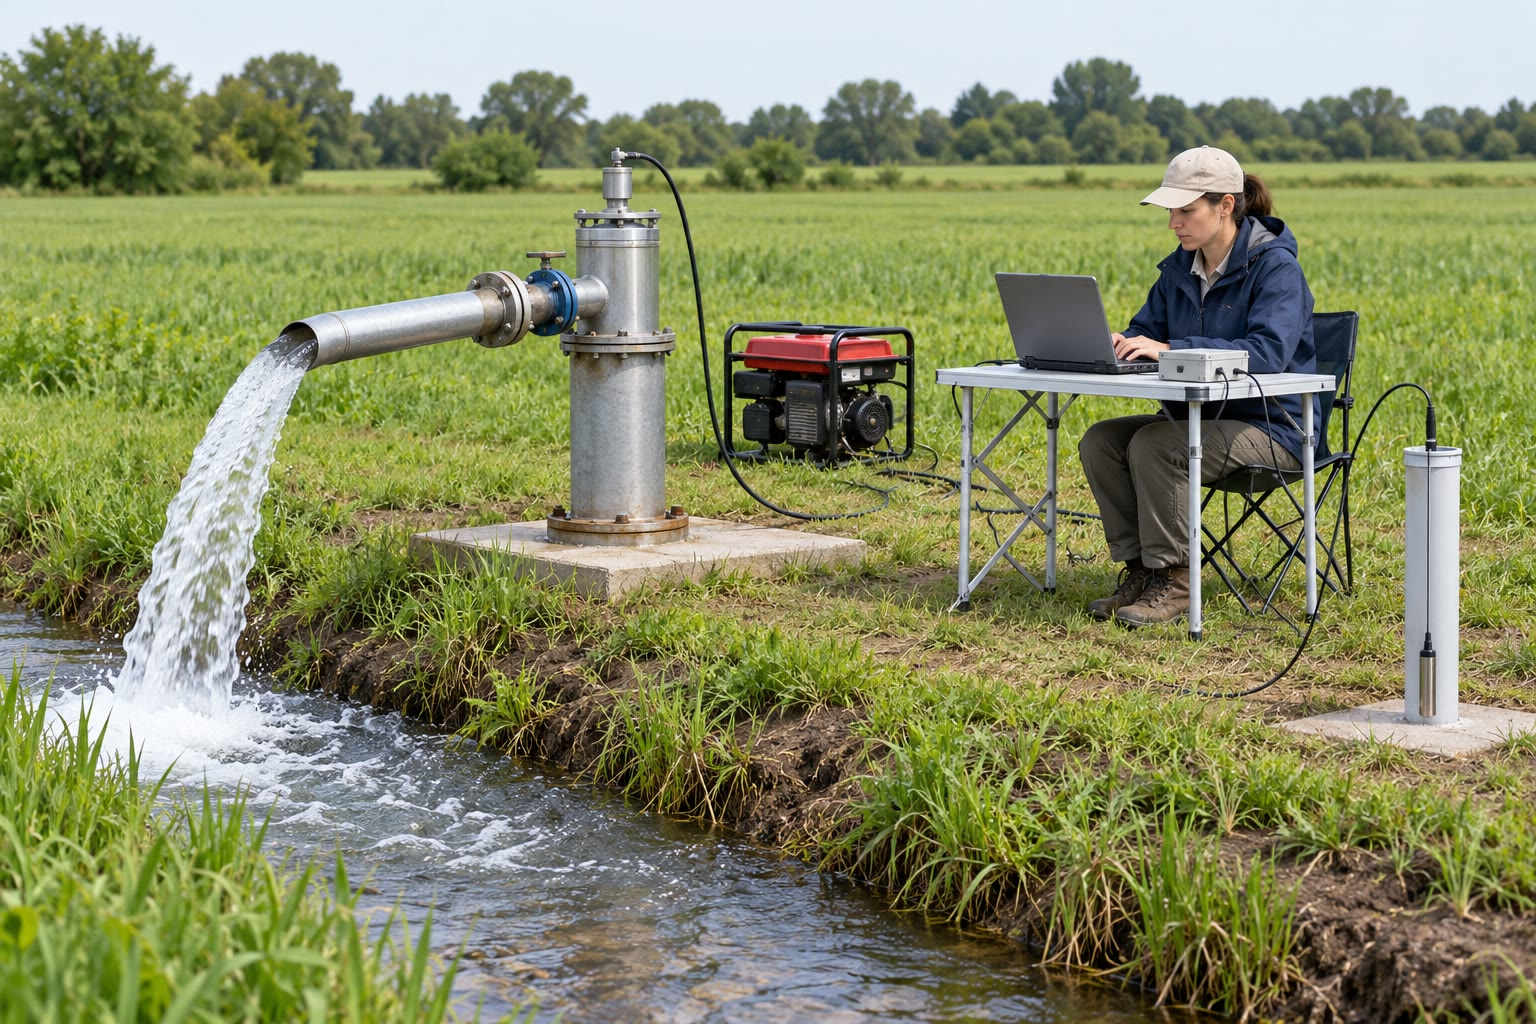
\includegraphics[width=\linewidth]{images/book5/ai/b3-pumping-test.jpg}

{\scriptsize اختبار الضخ: أنبوب التصريف للبئر التي يُضخّ منها، ومولِّد كهربائي،
وجيولوجيّ مائيّ يسجّل مناسيب بئر مراقبة على حاسوب محمول
(رسم توضيحي مولَّد بالذكاء الاصطناعي).}
\end{minipage}
\end{inthefield}
% ledger: heath:theis, heath:jacob, heath:water-levels, usgs:transducers

\section{انتقال المواد المذابة}\label{sec:b3:hydrogeology:transport}

تُنقل المادّة المذابة في المياه الجوفية مع الماء \omterm{def:b3:hydrogeology:seepage}{بسرعة التسرّب}،
وتنتشر أثناء حركتها: فالماء في المسام المجاورة
يتحرّك بسرعات ومسارات مختلفة، وتنتشر المادّة المذابة
بالانتشار أيضًا.

\begin{definition}[التشتّت الهيدروديناميكي؛ معامل التشتّت]\label{def:b3:hydrogeology:ade}
\emph{التشتّت الهيدروديناميكي}\index{التشتّت الهيدروديناميكي} هو
انتشار مادّة مذابة في المياه الجوفية المتدفّقة بفعل تغيّرات
سرعة الماء من مسامّةٍ إلى أخرى وبالانتشار الجزيئي. على امتداد
الجريان يُوصف بمعامل تشتّت $D = \alpha_Lv + D^*$،
حيث $v$ \omterm{def:b3:hydrogeology:seepage}{سرعة التسرّب}، و$D^*$ معامل الانتشار الجزيئي الفعّال،
و$\alpha_L$، وهو طول، يمثّل
\emph{معامل التشتّت}\index{معامل التشتّت} الطولي للوسط.
\end{definition}

\begin{theorem}[معادلة الانتقال الأفقي--التشتّت]\label{thm:b3:hydrogeology:ade}
على امتداد جريان أحادي البعد ذي سرعة تسرّب ثابتة $v$، يخضع
تركيز المادّة المذابة غير المتفاعلة $C(x, t)$ للمعادلة الآتية
\[
\frac{\partial C}{\partial t} = D\,\frac{\partial^2C}{\partial x^2} -
v\,\frac{\partial C}{\partial x} .
\]
إذا ثُبّت التركيز على $C_0$ عند $x = 0$ منذ $t = 0$، في وسطٍ
خالٍ في البداية من المادّة المذابة،
\[
\frac{C}{C_0} = \frac12\left[\operatorname{erfc}\frac{x - vt}{2\sqrt{Dt}} +
\mathrm e^{vx/D}\operatorname{erfc}\frac{x + vt}{2\sqrt{Dt}}\right] .
\]
\end{theorem}
\index{معادلة الانتقال الأفقي--التشتّت}

\begin{proof}
في شريحةٍ مساحة مقطعها الوحدة وطولها $\mathrm dx$، ذات
المسامية الفعّالة $n_e$، والمادّة المذابة المخزّنة هي $n_eC\,\mathrm dx$. ودفقها
$n_e(vC - D\,\partial C/\partial x)$، يُحمل مع الماء وينتشر بالتشتّت
كما ينتشر ما يصفه قانون فيك لمادّة منتشرة. ويُعطي حفظُ الكتلة
$n_e\partial_tC = -\partial_x[n_e(vC - D\partial_xC)]$، وهي المعادلة. ويُسلَّم هنا
بأنّ الصيغة تحقّقها وتحقّق الشروط؛
و\cref{exo:b3:hydrogeology:12} يتحقّق من انتشارها.
\end{proof}

في الإطار المتحرّك مع الماء، $\xi = x - vt$، تصبح المعادلة
معادلةَ الانتشار، وتتّسع الجبهة بمقدار $\sqrt{2Dt} = \sqrt{2\alpha_L
vt} = \sqrt{2\alpha_Lx}$: يزداد عرض الجبهة تناسبًا مع الجذر التربيعي
للمسافة المقطوعة.

\begin{definition}[عامل التأخير]\label{def:b3:hydrogeology:retardation}
مادّةٌ مذابة مُمتزّةٌ على الحبيبات، في حالة توازن وبتناسب مع تركيزها،
تتحرّك أبطأ من الماء. وعاملُ تأخيرها
\emph{عامل التأخير}\index{عامل التأخير (الامتزاز)} يُعطى بالعلاقة
\[
R = 1 + \frac{\rho_bK_d}{n} ,
\]
حيث $\rho_b$ هي الكثافة الحجمية الجافة للوسط، و$n$ مساميّتُه
و$K_d$ معامل التوزيع، أي الكتلة الممتزّة لكلّ وحدة كتلة من
المادّة الصلبة مقسومةً على التركيز في الماء. تتحرّك المادّة المذابة بسرعة $v/R$
وتتشتّت بالمعامل $D/R$.
\end{definition}

\begin{omfigure}
\begin{tikzpicture}
\begin{groupplot}[group style={group size=2 by 1, horizontal sep=1.5cm},
  width=0.48\linewidth, height=0.4\linewidth,
  tick label style={font=\scriptsize}, label style={font=\small}, title style={font=\small}]
\nextgroupplot[xlabel={الزمن (أيام)}, ylabel={التركيز النسبي $C/C_0$ عند \qty{100}{m}},
  xmin=0, xmax=1000, ymin=0, ymax=1.05, title={منحنيات الاختراق},
  legend style={font=\scriptsize, at={(0.97,0.03)}, anchor=south east}]
% computed in figdata/bachelor-3/advection_dispersion.py
\addplot[omDef, thick] table[x=t, y=c1] {figdata/out/bachelor-3-advection_dispersion-btc.dat};
\addlegendentry{$\alpha_L = \qty{1}{m}$}
\addplot[omMeth, thick] table[x=t, y=c3] {figdata/out/bachelor-3-advection_dispersion-btc.dat};
\addlegendentry{$\alpha_L = \qty{3}{m}$}
\addplot[omThm, thick] table[x=t, y=c10] {figdata/out/bachelor-3-advection_dispersion-btc.dat};
\addlegendentry{$\alpha_L = \qty{10}{m}$}
\addplot[black, thick, densely dashed, forget plot] table[x=t, y=cR] {figdata/out/bachelor-3-advection_dispersion-btc.dat};
\node[font=\scriptsize, anchor=west, align=left] at (axis cs:640,0.45) {$\alpha_L = \qty{3}{m}$,\\ $R = 3$};
\addplot[black!40, densely dotted, forget plot] coordinates {(200,0) (200,1.05)};
\nextgroupplot[xlabel={المسافة \babelsublr{(\unit{m})}}, ylabel={التركيز النسبي $C/C_0$ بعد 150 يومًا},
  xmin=0, xmax=160, ymin=0, ymax=1.05, title={قطاعات التركيز},
  legend style={font=\scriptsize, at={(0.03,0.03)}, anchor=south west}]
\addplot[omDef, thick] table[x=x, y=c1] {figdata/out/bachelor-3-advection_dispersion-profile.dat};
\addlegendentry{$\alpha_L = \qty{1}{m}$}
\addplot[omMeth, thick] table[x=x, y=c3] {figdata/out/bachelor-3-advection_dispersion-profile.dat};
\addlegendentry{$\alpha_L = \qty{3}{m}$}
\addplot[omThm, thick] table[x=x, y=c10] {figdata/out/bachelor-3-advection_dispersion-profile.dat};
\addlegendentry{$\alpha_L = \qty{10}{m}$}
\addplot[black!40, densely dotted, forget plot] coordinates {(75,0) (75,1.05)};
\end{groupplot}
\end{tikzpicture}

\par\smallskip{\small مادّة مذابة تُحقن باستمرار عند $x = 0$ في
جريانٍ بسرعة تسرّب \qty{0.5}{m/d}. يسارًا، التركيز
\qty{100}{m} في اتجاه انحدار التدرّج بدلالة الزمن: يصل الماء نفسه بعد
200 يومًا (بخط منقّط)؛ فكلّما كان \omterm{def:b3:hydrogeology:ade}{معامل التشتّت} أكبر، ظهرت الآثار الأولى
أبكر، وتأخّر بلوغ التركيز الكامل. وتصل مادّة مُمتزّة ذات $R =
3$ بعد ثلاثة أضعاف الزمن. ويمينًا، التركيز على طول الجريان بعد
150 يومًا، حين يكون الماء قد قطع \qty{75}{m}
(بخط منقّط).}\label{fig:b3:hydrogeology:transport}
\end{omfigure}

يصعب قياس معاملات التشتّت، وكثيرًا ما تُحدَّد عمليًّا بحسب
قواعد تقديرية. وأقدمها يأخذ \omterm{def:b3:hydrogeology:ade}{معامل التشتّت} الطولي عُشرَ
طول العمود. ويُظهر تجميعٌ لقياسات حقلية نُشر
عام 1992 أنّ \omterm{def:b3:hydrogeology:ade}{معامل التشتّت} يتزايد مع مقياس التجربة،
وأنّ القيم الموثوقة عند المقاييس الكبيرة قليلةٌ، وأنّها عند أيّ مقياس بعينه
تنتشر على رتبتين أو ثلاث من رتب القدر.
% ledger: epa:dispersivity

\section{التمارين}

\begin{exercise}[$\star$]\label{exo:b3:hydrogeology:1}
يقع بيزومتران متجاوران على أرض ترتفع \qty{120.0}{m} فوق
المستوى المرجعي. الأوّل مُصفّى عند عمق \qty{40}{m}، ويقف ماؤه
\qty{12.5}{m} تحت سطح الأرض؛ والثاني مُصفّى عند عمق \qty{80}{m}،
ويقف ماؤه \qty{15.0}{m} تحت سطح الأرض. احسب حمل الارتفاع
وحمل الضغط \omterm{def:b3:hydrogeology:head}{والحمل الهيدروليكي} عند موضعي التصفية. في أيّ اتجاه يجري
الماء بينهما، وتحت أيّ تدرّج رأسي؟
\end{exercise}

\begin{exercise}[$\star$]\label{exo:b3:hydrogeology:2}
عمودٌ من الرمل طوله \qty{50}{cm} وقطره \qty{10}{cm}، وله $K =
\qty{12}{m/d}$ ومسامية فعّالة قدرها 0.35، يمرّ فيه الماء تحت
فرقِ حمل قدره \qty{30}{cm}. احسب \omterm{def:b3:hydrogeology:darcy}{التصريف النوعي}، والتدفّق
بالليتر في الساعة، \omterm{def:b3:hydrogeology:seepage}{وسرعة التسرّب}.
\end{exercise}

\begin{exercise}[$\star$]\label{exo:b3:hydrogeology:3}
الحجر الجيري له $K = \qty{2.5}{m/d}$ للماء عند \qty{10}{\celsius}
($\rho = \qty{999.7}{kg/m^3}$، $\mu = \qty{1.306e-3}{Pa.s}$). احسب
\omterm{def:b3:hydrogeology:darcy}{النفاذية الذاتية} له، \omterm{def:b3:hydrogeology:darcy}{والموصلية الهيدروليكية} للماء عند
\qty{20}{\celsius} ($\rho = \qty{998.2}{kg/m^3}$، $\mu =
\qty{1.002e-3}{Pa.s}$).
\end{exercise}
% ledger: nist:water

\begin{exercise}[$\star$]\label{exo:b3:hydrogeology:4}
الحجر الجيري المحصور في فاردن-3 سُمكُه \qty{180}{m}، وله $K =
\qty{2.5}{m/d}$. احسب \omterm{def:b3:hydrogeology:storage}{الناقلية}، \omterm{def:b3:hydrogeology:storage}{ومعامل التخزين} الذي يكون له
لو أنّ تمدّد الماء وحده أطلق ماءً بمقدار \num{9e-7} لكلّ متر من الخزان الجوفي
لكلّ متر من الحمل. قارن بالقيمة $S = \num{2e-4}$.
\end{exercise}
% ledger: heath:storage

\begin{exercise}[$\star\star$]\label{exo:b3:hydrogeology:5}
بعد مدّة طويلة من الضخّ بمعدّل \qty{1500}{m^3/d}، توقّفت الانخفاضاتُ عن
التغيّر: \qty{2.35}{m} في بئر رصد يبعد \qty{20}{m} عن
بئر الضخّ، و\qty{0.82}{m} في بئر يبعد \qty{200}{m}. الخزان الجوفي
محصورٌ وسُمكُه \qty{40}{m}. احسب ناقليّتَه، \omterm{def:b3:hydrogeology:darcy}{والموصلية
الهيدروليكية} للخزان.
\end{exercise}

\begin{exercise}[$\star\star$]\label{exo:b3:hydrogeology:6}
بئرٌ تضخّ \qty{1200}{m^3/d} من \omterm{def:b3:hydrogeology:aquifer-types}{الخزان الجوفي المحصور} الذي له $T =
\qty{300}{m^2/d}$ و$S = \num{5e-4}$. احسب $u$، و$W(u)$ (من
السلسلة)، والانخفاض على بُعد \qty{300}{m} بعد 1 يوم وبعد 10 أيام.
\end{exercise}

\begin{exercise}[$\star\star$]\label{exo:b3:hydrogeology:7}
لاختبار فاردن-3 ($T = \qty{450}{m^2/d}$، $S = \num{2e-4}$)، بعد
كم دقيقةً يجوز استخدام خطّ كوبر--جاكوب في آبار الرصد
على بُعد \qty{60}{m} و\qty{500}{m} من بئر الضخّ؟ ماذا يقول هذا
عن المكان الذي ينبغي أن تُوضَع فيه آبار الرصد لاختبار قصير؟
\end{exercise}

\begin{exercise}[$\star\star$]\label{exo:b3:hydrogeology:8}
بئران تبعد إحداهما عن الأخرى \qty{400}{m} في الحجر الجيري في تلال فاردن، يضخّ كلٌّ منهما
\qty{2160}{m^3/d}. احسب الانخفاض بعد 10 أيام في منتصف المسافة بينهما،
وعند موقع البئر الثانية بسبب البئر الأولى وحدها. لماذا يكلّف ضخُّ كلّ بئر
البئرَ الأخرى مالًا؟
\end{exercise}

\begin{exercise}[$\star\star$]\label{exo:b3:hydrogeology:9}
في \omterm{def:b3:hydrogeology:flow-net}{شبكة الانسياب} تحت السدّ، عدّ قنوات الانسياب وانخفاضات الحمل.
مع $K = \qty{5}{m/d}$ و$H = \qty{10}{m}$، احسب التسرّب لكلّ
متر من السدّ وتحت سدّ طوله \qty{300}{m}.
\end{exercise}

\begin{exercise}[$\star\star\star$]\label{exo:b3:hydrogeology:10}
مثِّل الرمل النظيف بأنابيبَ مستقيمةٍ نصف قطرها \qty{50}{\micro\metre} ومسامية
0.30. احسب $k$ و$K$ (للماء عند \qty{20}{\celsius}، كما في
\cref{exo:b3:hydrogeology:3})،
وقارن النتيجة بمدى الرمل النظيف. أيّ خصائص للرمل الحقيقي لا يشملها النموذج،
وفي أيّ اتجاه تُغيّر كلٌّ منها $K$؟
\end{exercise}
% ledger: nist:water, heath:k-chart

\begin{exercise}[$\star\star\star$]\label{exo:b3:hydrogeology:11}
(أ)~أثبِت أنّ انخفاض كوبر--جاكوب يتلاشى عند $r_0 =
\sqrt{2.25\,Tt/S}$. (ب)~احسب $r_0$ بعد 30 يومًا من الضخّ في
الحجر الجيري المحصور في تلال فاردن، وللصخر نفسه غير المحصور، مع $S =
0.2$. (ج)~لماذا يمكن لمخروط \omterm{def:b3:hydrogeology:aquifer-types}{الخزان الجوفي المحصور} أن يبلغ حدًّا
لم يكن الاختبار يقصد رصده؟
\end{exercise}
% ledger: heath:jacob, heath:storage

\begin{exercise}[$\star\star\star$]\label{exo:b3:hydrogeology:12}
(أ)~عند مسافة انتقال طويلة يقترب منحنى الاختراق عند $x$ من توزيع
طبيعيّ بالنسبة إلى الزمن، متوسطه $x/v$ وانحرافه المعياري $\sigma_t
= \sqrt{2\alpha_Lx}/v$. أثبِت ذلك انطلاقًا من انتشار الجبهة $\sqrt{2Dt}$.
(ب)~عند \qty{100}{m}، ومع $v = \qty{0.5}{m/d}$، يبلغ التركيز
\qty{16}{\percent} بعد \num{152.6}~يومًا، و\qty{84}{\percent} بعد
\num{247.2}~يومًا. قدّر $\alpha_L$. (ج)~خزان جوفي رمليّ له $\rho_b =
\qty{1.9}{g/cm^3}$ و$n = 0.30$؛ ولمادةٍ مُذابة $K_d =
\qty{0.32}{cm^3/g}$. احسب $R$.
\end{exercise}

\section{مسألة: اختبار الضخّ في فاردن-3}

\begin{problem}[{مسألة نهاية الأسبوع --- الأحمال الهيدروليكية، واختبار الضخّ، وانتقال
ملوّث في الحجر الجيري المحصور في تلال فاردن}]
\label{pb:b3:hydrogeology:1}
حُفرت البئر المفترضة فاردن-3 عند \babelsublr{(4500, 5000)} على شبكة
تلال فاردن، انطلاقًا من منسوب أرضي قدره \qty{363.2}{m}، عبر
طفل الجوراسي حتى الحجر الجيري الجوراسي، ويقع أعلاه عند
\qty{282.5}{m} وقاعدته عند \qty{102.5}{m} فوق مستوى سطح البحر، والبئر مفتوحة
على كامل سُمك الحجر الجيري. قبل الاختبار يكون الماء فيها على عمق
\qty{45.0}{m} تحت سطح الأرض.

\medskip\noindent\textbf{الجزء الأول --- الخزان الجوفي وجريانه الطبيعي.}
\begin{enumerate}
\item احسب سُمك الطَّفل وسُمك الحجر الجيري عند البئر.
\item احسب الحمل في الحجر الجيري والحمل الضغطي عند قمّته.
  لماذا يُعدّ الحجر الجيري خزانًا جوفيًّا محصورًا هنا؟
\item ثلاثة مقاييس ضغط جوفي مفتوحة على الحجر الجيري، عند \babelsublr{P1 (4300, 5250)}،
  و\babelsublr{P2 (4850, 5150)} و\babelsublr{P3 (4550, 4650)}، بأحمال هيدروليكية 318.96 و317.34
  و\qty{317.52}{m}. بكتابة $h = ax + by + c$، أوجد $a$ و$b$.
\item احسب \omterm{def:b3:hydrogeology:head}{التدرّج الهيدروليكي} والسمت الذي يتّجه نحوه
  الماء.
\end{enumerate}

\medskip\noindent\textbf{الجزء الثاني --- اختبار الضخّ.} تُضخّ البئر
بمعدّل \qty{2160}{m^3/d} لمدّة يومين. وفي بئر رصد تبعد \qty{60}{m}
عنها تكون الانخفاضات كما يلي:
\begin{center}
\begin{tabular}{l*{11}{c}}
\hline
\mbox{\textdir TLT $t$ (\unit{min})} & 1 & 2 & 3 & 5 & 7 & 10 & 15 & 20 & 30 & 45 & 60\\
\mbox{\textdir TLT $s$ (\unit{m})} & 0.18 & 0.36 & 0.48 & 0.64 & 0.77 & 0.88 & 1.04 & 1.15 & 1.30 & 1.45 & 1.56\\
\hline
\mbox{\textdir TLT $t$ (\unit{min})} & 90 & 120 & 180 & 240 & 360 & 480 & 720 & 960 & 1440 & 2160 & 2880\\
\mbox{\textdir TLT $s$ (\unit{m})} & 1.71 & 1.82 & 1.98 & 2.08 & 2.24 & 2.35 & 2.50 & 2.61 & 2.77 & 2.92 & 3.03\\
\hline
\end{tabular}
\end{center}
\begin{enumerate}[resume]
\item ارسم $s$ بدلالة $\log_{10}t$. أيّ النقاط الأولى تخرج عن الخطّ
  المستقيم، ولماذا؟
\item من الجزء المستقيم، قِس الانخفاض لكلّ دورة لوغاريتمية.
\item احسب \omterm{def:b3:hydrogeology:storage}{الناقلية}.
\item أوجد الزمن $t_0$ الذي يلتقي عنده الخطّ بالانخفاض الصفري.
\item احسب \omterm{def:b3:hydrogeology:storage}{معامل التخزين}.
\item تحقّق من أنّ $u \le 0.05$ للنقاط المستخدمة.
\item احسب \omterm{def:b3:hydrogeology:darcy}{الموصلية الهيدروليكية} للحجر الجيري.
\end{enumerate}

\medskip\noindent\textbf{الجزء الثالث --- المخروط.} من هنا خذ $T =
\qty{450}{m^2/d}$ و$S = \num{2e-4}$.
\begin{enumerate}[resume]
\item احسب انخفاض ثيس في بئر الرصد بعد يومين
  وقارنه بالسجلّ.
\item بئر مزرعة تبعد \qty{1}{km} تستمدّ من الحجر الجيري نفسه. احسب
  انخفاضها بعد 30 يومًا من الضخّ.
\item احسب مسافة جاكوب $r_0$ بعد 30 يومًا. ماذا تقول عن
  حدود الخزان الجوفي وصدع تلال فاردن؟
\item احسب الحجم المضخوخ خلال 30 يومًا. من أين، في \omterm{def:b3:hydrogeology:aquifer-types}{الخزان الجوفي المحصور}،
  يأتي هذا الحجم؟
\item كيف يُقارَن انخفاض بئر المزرعة لو كان الحجر الجيري
  غير محصور، مع $S = 0.18$؟
\end{enumerate}

\medskip\noindent\textbf{الجزء الرابع --- ملوِّث.} يصل تسرّب لملوِّث مُذاب
إلى الحجر الجيري على بُعد \qty{200}{m} من البئر. خذ
مسامية فعّالة قدرها 0.18 \omterm{def:b3:hydrogeology:retardation}{وعامل تأخير} قدره 2.5.
\begin{enumerate}[resume]
\item قبل الضخّ، احسب \omterm{def:b3:hydrogeology:darcy}{التصريف النوعي} \omterm{def:b3:hydrogeology:seepage}{وسرعة
  التسرّب} للجريان الطبيعي في الجزء~الأول.
\item كم من الزمن يستغرق الماء لقطع \qty{200}{m}، وكم يستغرق
  الملوِّث؟
\item مع ضخّ البئر، والتسرّب واقع أعلى التدرّج منها، يصبح الجريان
  شعاعيًّا نحو البئر. أثبِت أنّ الماء يستغرق $t = \pi n_e b
  r^2/Q$ للوصول إلى البئر من مسافة $r$، مُهمِلًا الجريان الطبيعي،
  واحسب ذلك للماء وللملوِّث.
\item باعتماد القاعدة التقريبية القائلة إنّ \omterm{def:b3:hydrogeology:ade}{معامل التشتّت} يساوي عُشر المسافة،
  قدّر انتشار الجبهة $\sqrt{2\alpha_Lx}$ عند البئر. ماذا
  يعني ذلك بالنسبة إلى أوّل وصول؟
\item هل ينبغي أن يستمرّ الضخّ؟ أعطِ حجّةً واحدةً مؤيّدة وأخرى معارضة.
\item أعطِ ناقلية خزان الحجر الجيري في تلال فاردن، بالمتر المربّع
  في اليوم، بدقّة رقمين معنويّين.
\end{enumerate}
\end{problem}
% ledger: heath:jacob, heath:theis, heath:storage, epa:dispersivity, region:name
